% Del pipeline al procesador dual-issue (documento independiente).
% Compilar con ./build.sh (genera primero las figuras de ./figs).
\documentclass[11pt,a4paper]{article}
\usepackage[utf8]{inputenc}
\usepackage[T1]{fontenc}
\usepackage[spanish,es-noquoting,es-tabla,es-nolists]{babel}
\usepackage{lmodern}            % typewriter (instrucciones)
\usepackage{mathpazo}           % texto y matemáticas: Palatino
\usepackage[scale=0.9]{tgheros} % sans serif de títulos, pies de figura y figuras
\linespread{1.06}
\usepackage{microtype}
\usepackage[a4paper,margin=2.4cm]{geometry}
\usepackage{graphicx}
\usepackage{pdflscape}
\usepackage{booktabs}
\usepackage{array}
\usepackage{amsmath}
\usepackage{caption}
\usepackage{enumitem}
\usepackage{xcolor}
\usepackage{listings}
\usepackage[most]{tcolorbox}
\usepackage{titlesec}
\usepackage[hidelinks]{hyperref}

\graphicspath{{figs/}}
\definecolor{hhblue}{RGB}{11,111,184}
\definecolor{hzd}{RGB}{217,95,2}
\definecolor{new}{RGB}{21,128,61}

\captionsetup{labelfont={bf,sf,color=hhblue},textfont={bf,sf,small},labelsep=quad,
  figurename=Figura,tablename=Tabla}

% headings as in the book: sans bold, number in black, title in blue
\titleformat{\section}{\sffamily\bfseries\Large}{\thesection}{0.7em}{\color{hhblue}}
\titleformat{\subsection}{\sffamily\bfseries\large}{\thesubsection}{0.7em}{\color{hhblue}}
\titleformat{\paragraph}[runin]{\sffamily\bfseries\normalsize}{}{0pt}{\color{hhblue}}
\titlespacing*{\section}{0pt}{3.2ex plus 1ex minus .2ex}{1.6ex plus .2ex}
\titlespacing*{\subsection}{0pt}{2.6ex plus 1ex minus .2ex}{1.2ex plus .2ex}
\titlespacing*{\paragraph}{0pt}{1.6ex plus .5ex minus .2ex}{0.8em}

% signal names in italics (as in the book); lane number as subscript
\newcommand{\sig}[1]{\textit{#1}}
\newcommand{\sigk}[2]{\textit{#1}\textsubscript{#2}}
\newcommand{\ins}[1]{\texttt{#1}}

% HDL examples, numbered per chapter
\lstdefinestyle{vlog}{language=Verilog, basicstyle=\ttfamily\footnotesize, columns=fullflexible,
  keywordstyle=\color{hhblue}\bfseries, commentstyle=\color{black!55}\itshape,
  showstringspaces=false, keepspaces=true, upquote=true,
  breaklines=true, breakindent=0pt, breakautoindent=true}
\newcounter{hdl}
\newtcblisting{hdl}[1]{listing only, breakable, colback=black!3, colframe=black!35,
  boxrule=0.4pt, arc=1.5pt, left=4pt, right=4pt, top=2pt, bottom=2pt,
  title={\sffamily\footnotesize\refstepcounter{hdl}\textbf{\textcolor{hhblue}{Ejemplo HDL \thehdl}}\quad #1},
  coltitle=black, colbacktitle=black!10, listing options={style=vlog}}

\setlist{itemsep=1pt, topsep=3pt}
\setlist[itemize]{label=\textbullet}

\begin{document}

\begin{center}
  {\sffamily\bfseries\huge\color{hhblue} Del pipeline al procesador dual-issue\par}
  \vspace{0.6ex}
  {\sffamily\large Diseño de un RISC-V superescalar de dos vías, en orden\par}
  \vspace{1.2ex}
  \rule{\linewidth}{0.4pt}
\end{center}
\vspace{1ex}

Un procesador segmentado de cinco etapas puede completar, como máximo, una instrucción por
ciclo. Para superar ese límite hay que ejecutar varias instrucciones a la vez. Este
documento parte de un pipeline RISC-V de cinco etapas con manejo completo de hazards y lo
transforma, paso a paso, en un procesador \emph{superescalar dual-issue en orden}, capaz de
buscar, decodificar y ejecutar hasta \emph{dos} instrucciones por ciclo.

A partir de la sección~\ref{sec:lanes}, cada sección agrega una parte al datapath y
presenta la figura resultante, hasta llegar al procesador completo de la
Fig.~\ref{fig:proc-full}. Algunos bloques se detallan con fragmentos de Verilog (los
\emph{Ejemplos HDL}). Los diagramas de ejecución de las
secciones~\ref{sec:forward} a~\ref{sec:stallflush} provienen de simular ese mismo
hardware.

% =====================================================================
\section{El punto de partida: el pipeline de cinco etapas}
\label{sec:base}

La Fig.~\ref{fig:base} muestra el procesador de partida~\cite{harris}. Las instrucciones
avanzan por cinco etapas: \emph{Fetch} (F), \emph{Decode} (D), \emph{Execute} (E),
\emph{Memory} (M) y \emph{Writeback} (W). Las etapas están separadas por registros de
pipeline, y cada señal lleva como sufijo la etapa a la que pertenece: \sig{RdE}, por
ejemplo, es el registro destino de la instrucción que se encuentra en Execute.

\begin{figure}[htbp]
\centering
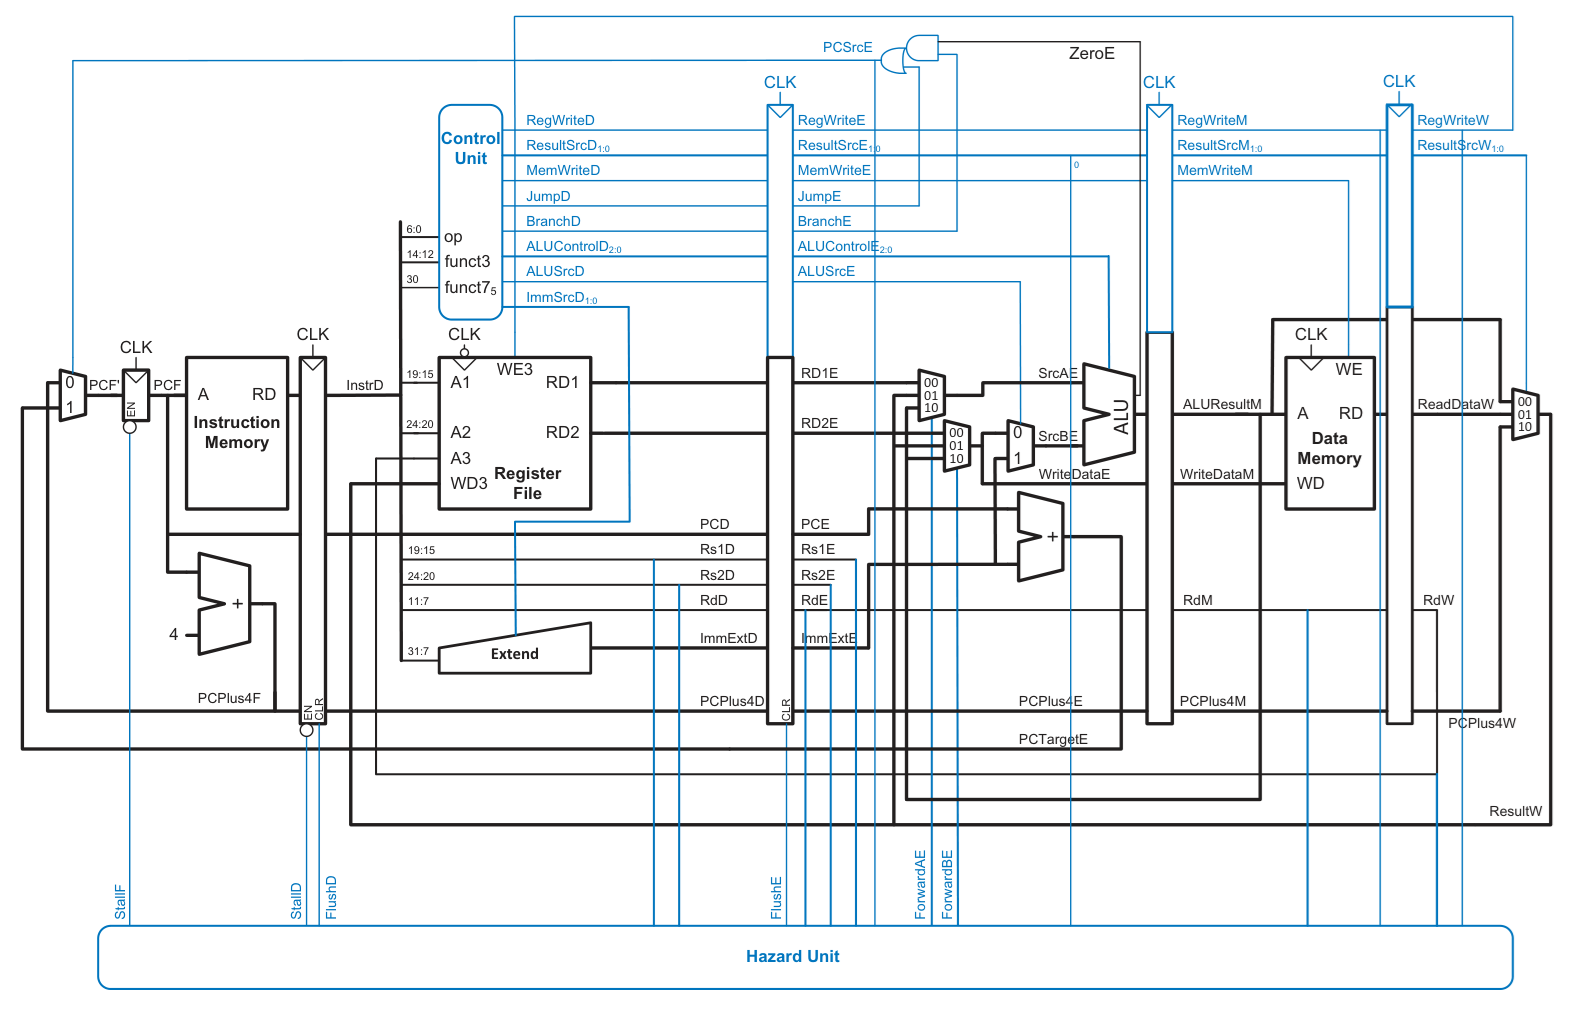
\includegraphics[width=\linewidth]{pipeline-base}
\caption{Procesador segmentado de cinco etapas con manejo de hazards (adaptado
de~\cite{harris})}
\label{fig:base}
\end{figure}

Como hay hasta cinco instrucciones en el pipeline al mismo tiempo, aparecen
\emph{hazards}: situaciones en las que una instrucción necesita un resultado que otra
todavía no ha producido. La Hazard Unit, en la parte inferior de la figura, los resuelve
con tres mecanismos:
\begin{itemize}
  \item \textbf{Forwarding.} Si una instrucción en Execute lee un registro que una
        instrucción anterior aún no ha escrito, el valor se toma directamente de la etapa
        Memory (\sig{ALUResultM}) o Writeback (\sig{ResultW}). \sig{ForwardAE} y
        \sig{ForwardBE} seleccionan la fuente; si ambas etapas contienen el registro, tiene
        prioridad Memory, porque guarda el valor más reciente.
  \item \textbf{Stall por load-use.} El dato de un \ins{lw} solo está disponible al final
        de la etapa Memory. Si la instrucción siguiente lo usa, el forwarding no basta:
        \sig{StallF} y \sig{StallD} detienen Fetch y Decode durante un ciclo, y
        \sig{FlushE} inserta una burbuja en Execute.
  \item \textbf{Flush por salto.} Los saltos se resuelven en Execute y se predicen como
        no tomados. Si el salto se toma (\sig{PCSrcE}), las dos instrucciones buscadas a
        continuación pertenecen al camino incorrecto y se descartan con \sig{FlushD} y
        \sig{FlushE}.
\end{itemize}
Además, el register file se escribe en la primera mitad del ciclo y se lee en la segunda,
de modo que una instrucción en Decode lee el valor que escribe otra que se encuentra en
Writeback.

Aun con estos mecanismos, el pipeline completa como máximo una instrucción por ciclo. En
términos del IPC (\emph{instructions per cycle}, el promedio de instrucciones completadas
por ciclo), esto significa que $\text{IPC} \le 1$ o, de forma equivalente,
$\text{CPI} \ge 1$.

% =====================================================================
\section{Visión general}
\label{sec:overview}

El pipeline aprovecha el \emph{paralelismo temporal}: varias instrucciones ocupan etapas
distintas al mismo tiempo, pero como máximo una entra a Execute en cada ciclo. Un
procesador superescalar agrega \emph{paralelismo espacial}: replica el hardware de
ejecución para que varias instrucciones avancen juntas por la misma etapa. El procesador
de este documento es de dos vías (\emph{two-way}) y \emph{en orden}: las instrucciones se
emiten en el orden del programa y una instrucción más joven nunca se adelanta a una más
antigua. Con dos vías, el IPC ideal es~2.

\paragraph{Terminología.} En el resto del documento se usan estos términos.
\begin{itemize}
  \item \textbf{Par}: las dos instrucciones consecutivas que se buscan y decodifican juntas.
  \item \textbf{Slot 0 / slot 1}: posición dentro del par. El slot~0 contiene siempre la
        instrucción \emph{más antigua} (dirección $\sig{PCD}_0$) y el slot~1 la
        \emph{más joven} ($\sig{PCD}_1 = \sig{PCD}_0 + 4$).
  \item \textbf{Vía} (\emph{lane}): cada una de las dos copias del camino de ejecución
        (Execute, Memory y Writeback). El slot~0 entra siempre a la vía~0 y el slot~1 a la
        vía~1; por lo tanto, \textbf{la vía~1 contiene siempre la instrucción más joven}.
        Todas las prioridades del diseño se derivan de esta propiedad.
  \item \textbf{Emitir} (\emph{issue}): pasar una instrucción de Decode a Execute. En cada
        ciclo se emiten dos instrucciones, una o ninguna.
\end{itemize}

\paragraph{Decisiones de diseño.} No conviene replicar todos los recursos. Una ALU es
barata, mientras que una memoria de datos de dos puertos o una segunda lógica de
resolución de saltos son caras y se usarían poco: en un programa típico, rara vez dos
instrucciones consecutivas acceden ambas a memoria o son ambas saltos. Por eso se fijan los
recursos de la Tabla~\ref{tab:resources}: casi todo el datapath se replica, pero la
memoria de datos y la \emph{Branch Unit}, que resuelve los saltos, son
\emph{compartidas}. Al compartirlas, hace falta una unidad que decida, en cada ciclo, qué
instrucciones se emiten.

\begin{table}[htbp]
\centering\small
\caption{Recursos del procesador dual-issue}
\label{tab:resources}
\begin{tabular}{@{}lll@{}}
\toprule
Recurso & Cantidad & Consecuencia \\
\midrule
Lectura de instrucciones & 2 por ciclo & memoria de instrucciones con dos puertos de lectura \\
Register file & 4 lecturas, 2 escrituras & un par completo lee y escribe en un ciclo \\
ALU & 2 & dos operaciones ALU por ciclo \\
Memoria de datos & 1 puerto & como máximo un \ins{lw}/\ins{sw} por par \\
Branch Unit & 1 & como máximo un \ins{beq}/\ins{jal} por par \\
Emisión & en orden & la más joven nunca se adelanta a la más antigua \\
\bottomrule
\end{tabular}
\end{table}

\paragraph{Diagramas de ejecución.} La ejecución se representa con diagramas como el de
la Fig.~\ref{fig:pd-pairs}. Cada fila corresponde a una instrucción y cada columna a un
ciclo. Cada celda indica el componente que la instrucción usa en ese ciclo: memoria de
instrucciones (IM), register file (RF), ALU, memoria de datos (DM) y, de nuevo, register
file en la escritura. La mitad sombreada del RF indica si se lee (segunda mitad del ciclo,
en Decode) o se escribe (primera mitad, en Writeback). Las flechas azules representan
forwarding, y la columna \textsf{v0}/\textsf{v1} indica la vía en la que se ejecuta cada
instrucción.

\begin{figure}[htbp]
\centering
\includegraphics[width=0.82\linewidth]{pd-pairs}
\caption{Tres pares emitidos en ciclos consecutivos; en el ciclo~5 las dos ALU operan
simultáneamente y el forwarding cruza entre vías}
\label{fig:pd-pairs}
\end{figure}

La Fig.~\ref{fig:pd-pairs} muestra el caso ideal: tres pares sin dependencias entre sus
instrucciones entran a Execute en ciclos consecutivos. En el ciclo~5, \ins{add x5} (vía~0)
recibe \ins{x1} de su propia vía y \ins{x2} de la vía~1, mientras que \ins{sub x6}
(vía~1) recibe \ins{x3} de la vía~0. Es decir, el forwarding ahora \emph{cruza entre
vías} (sección~\ref{sec:forward}).

El hardware se construye en cuatro pasos:
\begin{enumerate}
  \item replicar el datapath y compartir la memoria de datos y la Branch Unit
        (secciones~\ref{sec:lanes} y~\ref{sec:shared});
  \item extender el forwarding a las dos vías (sección~\ref{sec:forward});
  \item agregar la \emph{Issue Unit}, que decide cuántas instrucciones del par se emiten, y
        el mecanismo de reagrupamiento (sección~\ref{sec:issue});
  \item adaptar los stalls por \ins{lw} y los flushes por salto (sección~\ref{sec:stallflush}).
\end{enumerate}

Las figuras del datapath usan cinco colores: negro para los datos, azul para el control,
naranja para la Hazard Unit y sus señales, verde para la Issue Unit y morado para la
Branch Unit. Un punto indica una unión entre cables; dos cables que se cruzan sin punto no
están conectados.

% =====================================================================
\section{Datapath de dos vías}
\label{sec:lanes}

El primer paso consiste en construir el datapath de dos vías sin considerar aún los
hazards. La Fig.~\ref{fig:proc-1} muestra el resultado. La vía~0 (arriba) es el pipeline
de la Fig.~\ref{fig:base} sin la Hazard Unit, y la vía~1 (abajo) es su imagen especular.
Los elementos que comparten ambas vías se ubican sobre el eje central de la figura: la
memoria de instrucciones, el registro IF/ID, el register file, la memoria de datos y la
Branch Unit.

\subsection{Fetch doble}

La memoria de instrucciones tiene dos puertos de lectura que reciben la misma dirección
\sig{PCF}: $\sig{RD1} = \text{mem}[\sig{PCF}]$ entrega \sigk{InstrF}{0} y
$\sig{RD2} = \text{mem}[\sig{PCF}+4]$ entrega \sigk{InstrF}{1}. Como se buscan dos
instrucciones por ciclo, el PC avanza en~8 (\sig{PCPlus8F}) en lugar de~4.

Un único registro IF/ID de 192 bits almacena el par completo: las dos instrucciones
(\sigk{InstrD}{0}, \sigk{InstrD}{1}), sus direcciones ($\sigk{PCD}{0} = \sig{PCF}$,
$\sigk{PCD}{1} = \sig{PCPlus4F}$) y el $\sig{PC}+4$ de cada una
($\sigk{PCPlus4D}{0} = \sig{PCPlus4F}$, $\sigk{PCPlus4D}{1} = \sig{PCPlus8F}$), que se
calculan en Fetch y viajan con el par. Como es un solo registro, el par avanza o se detiene
completo, y así se mantiene el orden entre sus dos instrucciones.

\subsection{Decode doble y register file}

Cada slot tiene su propia unidad de control y su propio bloque Extend. Su $\sig{PC}+4$
(\sigk{PCPlus4D}{k}) no se calcula en Decode: llega ya hecho desde el registro IF/ID. El
register file debe atender al par completo
en un solo ciclo:
\begin{itemize}
  \item \textbf{cuatro puertos de lectura}: A1/A2 para el slot~0 y A4/A5 para el slot~1;
  \item \textbf{dos puertos de escritura}: A3/WD3/WE3 para la vía~0 y A6/WD6/WE6 para la vía~1.
\end{itemize}
Igual que en el pipeline de partida, la escritura ocurre en el flanco de bajada del
reloj. Aparece un caso nuevo: ambas vías pueden escribir \emph{el mismo} registro en el
mismo ciclo (dependencia WAW dentro del par). Como la vía~1 contiene siempre la instrucción más
joven, su valor es el que debe prevalecer: el puerto A6 se escribe después que A3 y, por
lo tanto, tiene prioridad.

\subsection{Las dos vías de Execute, Memory y Writeback}

Cada vía tiene sus propios registros ID/EX, EX/MEM y MEM/WB, su ALU y su multiplexor de
\sig{ResultW}. El sumador de \sig{PCTargetE}, en cambio, no se replica: forma parte de la
Branch Unit compartida (sección~\ref{sec:branchunit}). La Tabla~\ref{tab:regs} detalla el
contenido de cada registro, que coincide con el del pipeline de partida, replicado por vía
(sufijo~$k$). Los registros de control (en azul) también se replican: cada vía lleva sus
propias señales \sig{RegWrite}, \sig{ResultSrc}, \sig{MemWrite}, \sig{Jump}, \sig{Branch},
\sig{ALUControl} y \sig{ALUSrc}.

\begin{table}[htbp]
\centering\small
\caption{Registros de pipeline de cada vía ($k = 0, 1$)}
\label{tab:regs}
\begin{tabular}{@{}ll@{}}
\toprule
Registro & Contenido \\
\midrule
IF/ID (uno para el par) & \sigk{InstrD}{0}, \sigk{InstrD}{1}, \sigk{PCD}{0}, \sigk{PCD}{1}, \sigk{PCPlus4D}{0}, \sigk{PCPlus4D}{1} \\
ID/EX$_k$ & \sig{RD1}, \sig{RD2}, \sig{PC}, \sig{Rs1}, \sig{Rs2}, \sig{Rd}, \sig{ImmExt}, \sig{PCPlus4} \\
EX/MEM$_k$ & \sig{ALUResult}, \sig{WriteData}, \sig{Rd}, \sig{PCPlus4} \\
MEM/WB$_k$ & \sig{ALUResult}, \sig{ReadData}, \sig{Rd}, \sig{PCPlus4} \\
\bottomrule
\end{tabular}
\end{table}

\begin{hdl}{Memoria de instrucciones con dos puertos y escritura del register file}
// instruction memory: two consecutive words per cycle
assign rd1 = RAM[a[31:2]];      // InstrF_0 = mem[PCF]
assign rd2 = RAM[a[31:2]+1];    // InstrF_1 = mem[PCF+4]

// register file: two write ports, written in the first half of the cycle
always @(negedge clk) begin
  if (we3) rf[a3] <= wd3;       // lane 0
  if (we6) rf[a6] <= wd6;       // lane 1: same register -> the younger one wins
end
\end{hdl}

\begin{landscape}
\begin{figure}[p]
\centering
\includegraphics[width=\linewidth,height=0.88\textheight,keepaspectratio]{proc-1-lanes}
\caption{Paso 1: datapath de dos vías con fetch y decode dobles, register file de cuatro
lecturas y dos escrituras, memoria de datos compartida y Branch Unit compartida. Aún sin
manejo de hazards}
\label{fig:proc-1}
\end{figure}
\end{landscape}

% =====================================================================
\section{Recursos compartidos}
\label{sec:shared}

Ambas vías pueden recibir cualquier tipo de instrucción, por lo que cada recurso
compartido necesita multiplexores que lo asignen a la vía que lo requiere. Esto funciona
porque la Issue Unit (sección~\ref{sec:issue}) garantiza que un mismo par
\emph{nunca} contiene dos instrucciones de memoria ni dos saltos.

\subsection{Un solo puerto de memoria de datos}

La Fig.~\ref{fig:zoom-mem} muestra la etapa Memory. Dos multiplexores frente a la memoria
seleccionan la dirección (\sigk{ALUResultM}{k}) y el dato de escritura
(\sigk{WriteDataM}{k}) de la vía que contiene la instrucción de memoria. Su señal de
selección, \sig{MemLaneM}, vale~1 cuando la vía~1 contiene un \ins{lw} o un \ins{sw}; en
cualquier otro caso, el puerto se asigna a la vía~0. La señal de escritura es el OR de
ambas vías, ya que como máximo una de ellas escribe.

La lectura no requiere selección: \sig{ReadDataM} llega a los registros MEM/WB de
\emph{ambas} vías, y solo la vía que contiene el \ins{lw} lo utiliza, por ser la única con
$\sig{ResultSrcW} = 01$. En consecuencia, un par \ins{lw}~+~ALU se emite igual que un par
ALU~+~\ins{lw}: el orden dentro del par es indiferente.

\begin{hdl}{Puerto único de la memoria de datos}
assign MemWriteM = MemWriteM_0 | MemWriteM_1;              // at most one lane writes
assign MemLaneM  = MemWriteM_1 | (ResultSrcM_1 == 2'b01);  // lane 1 holds the lw/sw

mux2 #(32) memaddrmux(.d0(ALUResultM_0), .d1(ALUResultM_1), .s(MemLaneM), .y(ALUResultM));
mux2 #(32) memdatamux(.d0(WriteDataM_0), .d1(WriteDataM_1), .s(MemLaneM), .y(WriteDataM));
\end{hdl}

\begin{figure}[htbp]
\centering
\begin{minipage}[b]{0.47\linewidth}\centering
  \includegraphics[height=8.6cm]{proc-zoom-mem}
  \caption{Puerto único de la memoria de datos y su asignación a una vía}
  \label{fig:zoom-mem}
\end{minipage}\hfill
\begin{minipage}[b]{0.47\linewidth}\centering
  \includegraphics[height=8.6cm]{proc-zoom-branch}
  \caption{Branch Unit: recibe los operandos de ambas vías y genera \sig{PCSrcE},
  \sigk{TakenE}{0} y \sig{PCTargetE}}
  \label{fig:zoom-branch}
\end{minipage}
\end{figure}

\subsection{La Branch Unit}
\label{sec:branchunit}

En el pipeline de partida, el salto se resuelve en Execute mediante
$\sig{PCSrcE} = \sig{BranchE}\cdot\sig{ZeroE} + \sig{JumpE}$: la ALU compara los operandos
del \ins{beq} (señal \sig{Zero}) y un sumador dedicado calcula \sig{PCTargetE}. Replicar
esta lógica en cada vía produciría dos unidades de resolución, de las cuales nunca se
usaría más de una por ciclo. En su lugar, el diseño agrega un módulo único, la
\textbf{Branch Unit}, ubicado en el eje central del datapath (Fig.~\ref{fig:zoom-branch}).
Funciona en tres partes:
\begin{itemize}
  \item \textbf{Selección de la vía.} Como la Issue Unit nunca emite dos saltos en el
        mismo par, a lo sumo una vía tiene activa \sig{Branch} o \sig{Jump}. La señal
        $\sig{BrLaneE} = \sigk{BranchE}{1} + \sigk{JumpE}{1}$ controla cuatro
        multiplexores que toman los operandos de esa vía: \sig{PCE}, \sig{ImmExtE},
        \sig{SrcAE} y \sig{WriteDataE} (el valor de \sig{rs2}). Los dos últimos se toman
        después de los multiplexores de forwarding, de modo que el salto compara valores
        actualizados.
  \item \textbf{Resolución.} Un único comparador evalúa $\sig{SrcA} = \sig{SrcB}$, que
        reemplaza a la señal \sig{Zero} de la ALU, y un único sumador calcula
        $\sig{PCTargetE} = \sig{PCE} + \sig{ImmExtE}$. Las ALU dejan de participar en los
        saltos.
  \item \textbf{Salidas.} \sig{PCSrcE} y \sig{PCTargetE} van a la etapa Fetch, y
        \sig{PCSrcE} también a la Hazard Unit. Además, $\sigk{TakenE}{0} = \sig{PCSrcE}\cdot\overline{\sig{BrLaneE}}$
        indica que el salto tomado está en la vía~0; la Hazard Unit usa esta señal para
        anular la otra instrucción del par (sección~\ref{sec:branchflush}).
\end{itemize}
Como las señales \sig{Branch} y \sig{Jump} de las dos vías nunca están activas a la vez,
basta un OR para combinarlas, igual que la señal de escritura de la memoria de datos.

\begin{hdl}{Branch Unit (\texttt{branchunit.v})}
wire BrLaneE = BranchE_1 | JumpE_1;             // lane that holds the branch/jump

// operands of that lane (SrcAE / WriteDataE already forwarded)
mux2 #(32) pcmux (PCE_0,        PCE_1,        BrLaneE, PCE);
mux2 #(32) immmux(ImmExtE_0,    ImmExtE_1,    BrLaneE, ImmExtE);
mux2 #(32) amux  (SrcAE_0,      SrcAE_1,      BrLaneE, SrcAE);
mux2 #(32) bmux  (WriteDataE_0, WriteDataE_1, BrLaneE, SrcBE);

assign EqualE    = (SrcAE == SrcBE);            // one comparator
adder pcaddbranch(PCE, ImmExtE, PCTargetE);     // one target adder

assign PCSrcE    = ((BranchE_0 | BranchE_1) & EqualE) | JumpE_0 | JumpE_1;
assign TakenE_0  = PCSrcE & ~BrLaneE;           // taken branch/jump in lane 0
\end{hdl}

% =====================================================================
\section{Hazards de datos entre vías: forwarding}
\label{sec:forward}

El datapath de la Fig.~\ref{fig:proc-1} presenta los mismos hazards RAW que el pipeline de
partida, pero con más casos: una instrucción puede necesitar un resultado que aún está
en Memory o Writeback de su propia vía \emph{o de la otra}. La solución es la misma:
adelantar el valor desde la etapa en que se encuentra. La diferencia es que ahora hay
cuatro fuentes posibles en lugar de dos: \sigk{ALUResultM}{0}, \sigk{ALUResultM}{1},
\sigk{ResultW}{0} y \sigk{ResultW}{1}.

Estas cuatro señales forman un \emph{bus de forwarding} vertical que cruza el eje central
(Fig.~\ref{fig:zoom-fwd}) y llega a ambas vías. Los multiplexores frente a cada ALU pasan
de tres a cinco entradas, y \sig{ForwardAE} y \sig{ForwardBE} pasan de dos a tres bits
(Tabla~\ref{tab:fwd}). La Fig.~\ref{fig:proc-2} muestra el datapath con este cambio. La
Hazard Unit aparece en naranja, por ahora solo con sus entradas y sus salidas de
forwarding.

\begin{table}[htbp]
\centering\small
\caption{Códigos de \sigk{ForwardAE}{k} y \sigk{ForwardBE}{k}}
\label{tab:fwd}
\begin{tabular}{@{}cll@{}}
\toprule
Código & Fuente & Condición (en orden de prioridad) \\
\midrule
\texttt{100} & \sigk{ALUResultM}{1} & $\sig{Rs} = \sigk{RdM}{1}$ y \sigk{RegWriteM}{1} \\
\texttt{011} & \sigk{ALUResultM}{0} & $\sig{Rs} = \sigk{RdM}{0}$ y \sigk{RegWriteM}{0} \\
\texttt{010} & \sigk{ResultW}{1}    & $\sig{Rs} = \sigk{RdW}{1}$ y \sigk{RegWriteW}{1} \\
\texttt{001} & \sigk{ResultW}{0}    & $\sig{Rs} = \sigk{RdW}{0}$ y \sigk{RegWriteW}{0} \\
\texttt{000} & register file (\sig{RD1E}/\sig{RD2E}) & ninguna de las anteriores, o $\sig{Rs} = \texttt{x0}$ \\
\bottomrule
\end{tabular}
\end{table}

\paragraph{Prioridad.} En el pipeline de partida, si ambas etapas contienen el registro
buscado, tiene prioridad Memory, porque guarda el valor más reciente. Con dos vías se
agrega una segunda regla: \emph{dentro de una misma etapa tiene prioridad la vía~1},
porque contiene la instrucción más joven del par. El orden resultante es el de la tabla:
M$_1$, M$_0$, W$_1$, W$_0$. Por ejemplo, en el siguiente código:
\begin{center}\small
\begin{tabular}{@{}ll@{}}
\ins{addi x3, x0, 10} & \# par: vía 0 \\
\ins{addi x3, x0, 30} & \# par: vía 1 \\
\ins{add  x4, x3, x0} & \\
\ins{nop} & \\
\ins{addi x5, x3, 1}  & \\
\end{tabular}
\end{center}
El \ins{add} encuentra \ins{x3} en ambas vías de Memory y debe tomar el valor~30, de la
vía~1. Dos instrucciones después, \ins{addi x5} encuentra \ins{x3} en ambas vías de
Writeback y vuelve a seleccionar la vía~1, de modo que $\ins{x5} = 31$. Es la misma regla
que aplica el register file al escribir (A6 tiene prioridad sobre A3).

\begin{figure}[htbp]
\centering
\includegraphics[height=8.2cm]{proc-zoom-fwd}
\caption{Bus de forwarding entre vías: las cuatro fuentes (W0, W1, M0, M1) llegan a los
multiplexores de cinco entradas de ambas vías}
\label{fig:zoom-fwd}
\end{figure}

\begin{hdl}{Selección de la fuente de forwarding}
// youngest producer first: MEM before WB and, inside a stage, lane 1 before lane 0
function [2:0] fwd(input [4:0] rs, input [4:0] rdM1, rdM0, rdW1, rdW0,
                   input       weM1, weM0, weW1, weW0);
  if      (rs == 5'b0)            fwd = 3'b000;
  else if ((rs == rdM1) & weM1)   fwd = 3'b100;
  else if ((rs == rdM0) & weM0)   fwd = 3'b011;
  else if ((rs == rdW1) & weW1)   fwd = 3'b010;
  else if ((rs == rdW0) & weW0)   fwd = 3'b001;
  else                            fwd = 3'b000;
endfunction
\end{hdl}

\begin{landscape}
\begin{figure}[p]
\centering
\includegraphics[width=\linewidth,height=0.88\textheight,keepaspectratio]{proc-2-forward}
\caption{Paso 2: forwarding entre vías. Bus de cuatro fuentes, multiplexores de cinco
entradas y Hazard Unit (solo forwarding)}
\label{fig:proc-2}
\end{figure}
\end{landscape}

% =====================================================================
\section{La Issue Unit}
\label{sec:issue}

\subsection{Dependencias que el forwarding no resuelve}

El forwarding adelanta un resultado desde una etapa \emph{posterior}. Sin embargo, las dos
instrucciones de un par se encuentran en la \emph{misma} etapa: si el slot~1 necesita el
resultado del slot~0, ese valor se calcula en la otra ALU en el mismo ciclo en que el
slot~1 lo requiere, y no existe una etapa posterior desde la cual adelantarlo. Algo
similar ocurre con los recursos compartidos de la sección~\ref{sec:shared}: dos accesos a
memoria o dos saltos en el mismo par no pueden atenderse en un solo ciclo.

En estos casos, la instrucción más joven no puede emitirse en ese ciclo. La decisión la
toma un bloque nuevo, la \textbf{Issue Unit} (en verde en las figuras).

\subsection{Definición}

La Issue Unit es un bloque combinacional que, en Decode, examina el par y las
instrucciones que se encuentran en Execute, y determina cuántas instrucciones del par se
emiten:
\begin{itemize}
  \item \textbf{dos}: el caso normal;
  \item \textbf{una} (solo el slot~0): el slot~1 tiene un conflicto con el slot~0 o
        depende de un \ins{lw} que está en Execute. Se activa \sig{IssueOneD};
  \item \textbf{ninguna}: el slot~0 depende de un \ins{lw} que está en Execute. Se activa
        \sigk{LoadUseD}{0} y la Hazard Unit detiene el par completo
        (sección~\ref{sec:stallflush}).
\end{itemize}
Sus entradas son las dos instrucciones del par (\sigk{InstrD}{0}, \sigk{InstrD}{1}) y,
para detectar el load-use, el registro destino y el bit $\sig{ResultSrcE}[0]$ (igual a~1
para un \ins{lw}) de cada vía de Execute. Sus dos salidas van a la Hazard Unit, que las
convierte en las señales de control del pipeline.

La Issue Unit decodifica por su cuenta qué registros usa \emph{realmente} cada instrucción
(Tabla~\ref{tab:use}). Si comparara los campos \sig{rs1} y \sig{rs2} sin considerar el
tipo de instrucción, detectaría dependencias falsas, y cada una dividiría un par
innecesariamente. Por ejemplo, los bits 24:20 de un \ins{addi} forman parte del inmediato
y no designan un registro: sin esta tabla, un \ins{addi} cuyo inmediato coincidiera con el
\sig{rd} del slot~0 se trataría como dependiente.

\begin{table}[htbp]
\centering\small
\caption{Registros que usa cada tipo de instrucción, según la Issue Unit}
\label{tab:use}
\begin{tabular}{@{}lccc@{}}
\toprule
Instrucción & lee \sig{rs1} & lee \sig{rs2} & escribe \sig{rd} \\
\midrule
tipo R (\ins{add}, \ins{sub}, \ins{and}, \ins{or}, \ins{xor}, \ins{slt}) & sí & sí & sí \\
tipo I (\ins{addi}, \dots) & sí & no & sí \\
\ins{lw} & sí & no & sí \\
\ins{sw} & sí & sí & no \\
\ins{beq} & sí & sí & no \\
\ins{jal} & no & no & sí \\
\bottomrule
\end{tabular}
\end{table}

\subsection{Condiciones de emisión}

Con esa decodificación, la Issue Unit evalúa cuatro condiciones para el slot~1 y
una para el slot~0 (Tabla~\ref{tab:issue}).

\begin{table}[htbp]
\centering\small
\caption{Condiciones de la Issue Unit}
\label{tab:issue}
\begin{tabular}{@{}l>{\raggedright\arraybackslash}p{6.4cm}>{\raggedright\arraybackslash}p{4.6cm}@{}}
\toprule
Señal & Se activa cuando & Ejemplo \\
\midrule
\sig{rawD} & el slot~0 escribe un registro ($\neq$ \ins{x0}) que el slot~1 lee (RAW dentro del par) &
  \ins{addi x1,x0,5} / \ins{addi x2,x1,1} \\[1pt]
\sig{memD} & ambos slots acceden a memoria (un solo puerto) & \ins{sw} / \ins{sw}, \ins{lw} / \ins{sw} \\
\sig{ctrlD} & ambos slots son saltos (una sola Branch Unit) & \ins{beq} / \ins{beq}, \ins{beq} / \ins{jal} \\
\sigk{luseD}{1} & el slot~1 lee el destino de un \ins{lw} que está en Execute (en cualquier vía) & \ins{lw x4} en EX; slot~1 = \ins{add x5,x3,x4} \\
\midrule
\sig{IssueOneD} & $\sig{rawD} + \sig{memD} + \sig{ctrlD} + \sigk{luseD}{1}$ & se emite solo el slot~0 \\
\sigk{LoadUseD}{0} & el slot~0 lee el destino de un \ins{lw} que está en Execute (en cualquier vía) & no se emite ninguna \\
\bottomrule
\end{tabular}
\end{table}

Conviene notar tres cosas:
\begin{itemize}
  \item Solo importa el RAW del slot~1 respecto del slot~0; el caso inverso no puede
        ocurrir, porque el slot~0 es más antiguo. Las dependencias WAR y WAW dentro del
        par no impiden la emisión. WAR no genera conflicto porque ambos slots leen sus
        operandos antes de que cualquiera escriba, y WAW queda resuelta por la prioridad de
        la vía~1 en el register file y en el forwarding.
  \item \sig{memD} y \sig{ctrlD} solo se activan si \emph{ambos} slots usan el recurso.
        Una instrucción de memoria o un salto puede emitirse en cualquiera de los dos slots
        junto con una instrucción ALU, en cualquier orden; los multiplexores de la
        sección~\ref{sec:shared} asignan el recurso a la vía correspondiente.
  \item Si el slot~1 depende de un \ins{lw} en Execute, el slot~0 puede avanzar
        (\sigk{luseD}{1} solo divide el par). Si el que depende es el slot~0, no se emite
        ninguna instrucción, porque el slot~1 no puede adelantarse a él.
\end{itemize}

\begin{hdl}{Condiciones de la Issue Unit}
// RAW inside the pair: slot 1 needs the result of slot 0 in the same cycle (cannot forward)
wire rawD   = writes_0 & ((useRs1_1 & (rs1_1 == rd_0)) | (useRs2_1 & (rs2_1 == rd_0)));
// structural: one data memory port, one branch unit
wire memD   = mem_0  & mem_1;
wire ctrlD  = ctrl_0 & ctrl_1;

// load-use with a lw in Execute (either lane)
wire luseD_1 = loaduse(rs1_1, rs2_1, useRs1_1, useRs2_1, RdE_0, RdE_1, ResultSrcEb0_0, ResultSrcEb0_1);
assign LoadUseD_0 = loaduse(rs1_0, rs2_0, useRs1_0, useRs2_0, RdE_0, RdE_1, ResultSrcEb0_0, ResultSrcEb0_1);
assign IssueOneD  = rawD | memD | ctrlD | luseD_1;
\end{hdl}

\subsection{Emisión parcial y reagrupamiento}

Cuando solo se emite el slot~0, el slot~1 no debe perderse ni ejecutarse dos veces: debe
permanecer en Decode y emitirse en un ciclo posterior, sin alterar el orden del programa.
Hay dos alternativas:
\begin{enumerate}
  \item detener el par completo y repetirlo con el slot~0 convertido en burbuja;
  \item \emph{reagrupar}: la instrucción en espera pasa a ser el slot~0 del siguiente par,
        que se completa con la instrucción siguiente del programa.
\end{enumerate}
La primera es más simple, pero desperdicia un ciclo de cada vía en cada conflicto. El
diseño adopta la segunda (Fig.~\ref{fig:zoom-fetch}). La Hazard Unit genera
\[
  \sig{RegroupD} = \sig{IssueOneD}\cdot\overline{\sig{lwStallD}}\cdot\overline{\sig{PCSrcE}},
\]
y \sig{RegroupD} controla siete multiplexores en Fetch: seis frente al registro IF/ID (la
instrucción, el \sig{PC} y el $\sig{PC}+4$ de cada slot) y uno para el siguiente PC:
\begin{itemize}
  \item \textbf{nuevo slot~0} $\leftarrow$ el slot~1 actual (\sigk{InstrD}{1},
        \sigk{PCD}{1}, \sigk{PCPlus4D}{1}), realimentado desde la salida de IF/ID;
  \item \textbf{nuevo slot~1} $\leftarrow$ \sigk{InstrF}{0} = mem[\sig{PCF}], con dirección
        \sig{PCF} y $\sig{PC}+4$ igual a \sig{PCPlus4F};
  \item \textbf{siguiente PC} $\leftarrow$ $\sig{PCF} + 4$ en lugar de $\sig{PCF} + 8$.
\end{itemize}

\sigk{InstrF}{0} es justamente la instrucción que sigue al slot~1. Mientras un par
($\sig{PCD}_0$, $\sig{PCD}_0{+}4$) está en Decode, Fetch se encuentra en
$\sig{PCF} = \sig{PCD}_0 + 8 = \sig{PCD}_1 + 4$. El nuevo par queda formado por
($\sig{PCD}_1$, $\sig{PCD}_1 {+} 4$), es decir, por dos instrucciones consecutivas. Al
avanzar el PC solo en~4, Fetch queda en $\sig{PCD}_1 + 8$, alineado con el nuevo par. La
instrucción en espera siempre vuelve a entrar por el slot~0, de modo que la vía~1 sigue
conteniendo la más joven. En el mismo ciclo, \sigk{FlushE}{1} inserta una burbuja en la
vía~1, porque el slot~1 no se emitió.

\begin{figure}[htbp]
\centering
\includegraphics[height=12.5cm]{proc-zoom-fetch}
\caption{Fetch con reagrupamiento: \sig{RegroupD} elige entre el par recién buscado y el
slot~1 en espera (lazo \sigk{InstrD}{1}, \sigk{PCD}{1}, \sigk{PCPlus4D}{1}), y entre $\sig{PC}+8$ y
$\sig{PC}+4$}
\label{fig:zoom-fetch}
\end{figure}

La Fig.~\ref{fig:pd-raw} muestra el caso más simple:
\begin{itemize}
  \item \textbf{Ciclo~2.} \ins{addi x2, x1, 1} necesita el valor de \ins{x1} que calcula
        la otra instrucción del par, por lo que \sig{rawD} la retiene en Decode (celda
        rayada).
  \item \textbf{Ciclo~3.} Se reagrupa con \ins{addi x3} y el nuevo par se emite completo.
        \ins{x1} ya está en Memory y llega por forwarding.
  \item \textbf{Ciclo~5.} El par siguiente (\ins{add x4}, \ins{sub x5}) toma sus operandos
        de ambas vías a la vez.
\end{itemize}
La Fig.~\ref{fig:pd-regroup} repite el mecanismo varias veces seguidas, con una cadena de
incrementos de \ins{x1} intercalada con instrucciones independientes. Cada \ins{sw} guarda
el valor actual de \ins{x1}, de modo que una instrucción perdida o duplicada alteraría la
secuencia de valores en memoria.

\begin{figure}[htbp]
\centering
\includegraphics[width=0.85\linewidth]{pd-raw}
\caption{RAW dentro del par: solo se emite el slot~0, y \ins{addi x2} se reagrupa con la
instrucción siguiente}
\label{fig:pd-raw}
\end{figure}

\begin{figure}[htbp]
\centering
\includegraphics[width=0.85\linewidth]{pd-regroup}
\caption{Emisiones parciales repetidas. Las instrucciones rayadas esperan en Decode y se
emiten en la vía~0 del ciclo siguiente}
\label{fig:pd-regroup}
\end{figure}

\begin{hdl}{Selección del siguiente PC y reagrupamiento frente a IF/ID}
// next PC: PC+8 (pair issued), PC+4 (regroup) or the branch target
mux3 #(32) pcmux(.d0(PCPlus4F), .d1(PCTargetE), .d2(PCPlus8F),
                 .s({~PCSrcE & ~RegroupD, PCSrcE}), .y(PCNextF));

// Regroup: slot 1 (still not executed) becomes the new slot 0 and the
// instruction at PCF (= PCD_1 + 4) becomes the new slot 1.
wire [31:0] InstrN_0   = RegroupD ? InstrD_1   : InstrF_0;
wire [31:0] InstrN_1   = RegroupD ? InstrF_0   : InstrF_1;
wire [31:0] PCN_0      = RegroupD ? PCD_1      : PCF;
wire [31:0] PCN_1      = RegroupD ? PCF        : PCPlus4F;
wire [31:0] PCPlus4N_0 = RegroupD ? PCPlus4D_1 : PCPlus4F;
wire [31:0] PCPlus4N_1 = RegroupD ? PCPlus4F   : PCPlus8F;
\end{hdl}

\begin{landscape}
\begin{figure}[p]
\centering
\includegraphics[width=\linewidth,height=0.88\textheight,keepaspectratio]{proc-3-issue}
\caption{Paso 3: Issue Unit (verde) y reagrupamiento del par. \sig{IssueOneD} genera
\sig{RegroupD} y la burbuja \sigk{FlushE}{1} en la vía~1}
\label{fig:proc-3}
\end{figure}
\end{landscape}

% =====================================================================
\section{Stalls y control hazards}
\label{sec:stallflush}

Faltan los dos mecanismos del pipeline de partida que el forwarding no cubre: el stall por
\ins{lw} y el flush por salto tomado. Ambos se conservan, con ajustes para el par.

\subsection{Load-use}

Un \ins{lw} entrega su dato al final de Memory, por lo que la instrucción que lo usa a
continuación debe esperar un ciclo. Con dos vías, el \ins{lw} puede estar en cualquiera de
ellas y el consumidor en cualquiera de los dos slots:
\begin{itemize}
  \item si el consumidor es el \textbf{slot~0} (\sigk{LoadUseD}{0}), se detiene el par
        completo: \sig{StallF} y \sig{StallD} congelan el PC y el registro IF/ID, y
        \sigk{FlushE}{0} y \sigk{FlushE}{1} insertan una burbuja en ambas vías;
  \item si el consumidor es solo el \textbf{slot~1} (\sigk{luseD}{1}), el slot~0 se emite y
        el slot~1 se reagrupa, como se describió en la sección anterior.
\end{itemize}
La Fig.~\ref{fig:pd-loaduse} muestra el primer caso. \ins{lw x4} se ejecuta en la vía~1,
junto con un \ins{addi} independiente en la vía~0. El par siguiente comienza con
\ins{add x5, x3, x4}, que necesita \ins{x4}. Ambas instrucciones del par esperan un ciclo
en Decode, y en el ciclo~5 \ins{x4} llega desde Writeback de la vía~1. \ins{sw x5}, que
está en Fetch, también espera un ciclo.

Si el \ins{lw} y su consumidor quedan \emph{en el mismo par}, actúa primero \sig{rawD}: el
consumidor se reagrupa como slot~0. En el ciclo siguiente, el \ins{lw} está en Execute y
se activa \sigk{LoadUseD}{0}.

\begin{figure}[htbp]
\centering
\includegraphics[width=0.85\linewidth]{pd-loaduse}
\caption{Load-use con el \ins{lw} en la vía~1: el par completo espera un ciclo y se
inserta una burbuja en ambas vías}
\label{fig:pd-loaduse}
\end{figure}

\subsection{Saltos en cualquier posición del par}
\label{sec:branchflush}

Como en el pipeline de partida, el salto se resuelve en Execute y se predice como no
tomado. La diferencia es que lo resuelve la Branch Unit, que atiende a la vía en la que
se encuentre el salto. Cuando el salto se toma (\sig{PCSrcE}), la Branch Unit entrega la
dirección de destino (\sig{PCTargetE}) a Fetch, y las instrucciones buscadas después del
salto pertenecen al camino incorrecto y deben descartarse:
\begin{itemize}
  \item el par que está en Decode, con \sigk{FlushE}{0} y \sigk{FlushE}{1};
  \item el par que está en Fetch, con \sig{FlushD}.
\end{itemize}
Además, el salto puede compartir el par con otra instrucción, y en ese caso el tratamiento
depende del slot que ocupa (Fig.~\ref{fig:pd-branch}):
\begin{itemize}
  \item \textbf{Salto en el slot~0} (vía~0): la otra instrucción del par, en la vía~1, es
        \emph{más joven} y, por lo tanto, también pertenece al camino incorrecto. Como ya
        está en Execute, se anula al pasar a Memory mediante
        $\sigk{FlushM}{1} = \sigk{TakenE}{0}$, señal que genera la Branch Unit. Es el
        único registro EX/MEM que requiere entrada \sig{CLR}.
  \item \textbf{Salto en el slot~1} (vía~1): la otra instrucción del par, en la vía~0, es
        \emph{más antigua} y debe completarse normalmente. \sigk{FlushM}{1} no se activa,
        porque $\sigk{TakenE}{0} = 0$.
\end{itemize}

Por último, un salto tomado tiene prioridad sobre el load-use: si el par en Decode
pertenece al camino incorrecto, detenerlo no tiene sentido. Por ello la Hazard Unit usa
$\sig{lwStallD} = \sigk{LoadUseD}{0}\cdot\overline{\sig{PCSrcE}}$. Por la misma razón,
\sig{RegroupD} se anula cuando \sig{PCSrcE} está activa.

\begin{figure}[htbp]
\centering
\includegraphics[width=\linewidth]{pd-branch}
\caption{Saltos tomados en el slot~0 y en el slot~1. Las celdas grises tachadas son
instrucciones del camino incorrecto que se descartan; las que escriben~99 en \ins{x3}
nunca llegan a Writeback}
\label{fig:pd-branch}
\end{figure}

\subsection{Resumen de la Hazard Unit}

La Tabla~\ref{tab:hu} compara las ecuaciones de la Hazard Unit del pipeline de partida con
las del procesador dual-issue. Las señales \sig{PCSrcE} y \sigk{TakenE}{0} provienen de la
Branch Unit, y el forwarding se calcula igual para ambas vías, con la función de la
sección~\ref{sec:forward}. La Fig.~\ref{fig:proc-full} muestra el procesador completo.

\begin{table}[htbp]
\centering\small
\caption{Salidas de la Hazard Unit: pipeline de partida y dual-issue}
\label{tab:hu}
\renewcommand{\arraystretch}{1.15}
\begin{tabular}{@{}lll@{}}
\toprule
Salida & Pipeline de partida & Dual-issue \\
\midrule
\sig{lwStallD} & $\sig{ResultSrcE}_0\cdot(\sig{Rs1D}{=}\sig{RdE} + \sig{Rs2D}{=}\sig{RdE})$
               & $\sigk{LoadUseD}{0}\cdot\overline{\sig{PCSrcE}}$ \\
\sig{StallF}, \sig{StallD} & \sig{lwStallD} & \sig{lwStallD} \\
\sig{RegroupD} & --- & $\sig{IssueOneD}\cdot\overline{\sig{lwStallD}}\cdot\overline{\sig{PCSrcE}}$ \\
\sig{FlushD} & \sig{PCSrcE} & \sig{PCSrcE} \\
\sigk{FlushE}{0} & $\sig{lwStallD} + \sig{PCSrcE}$ & $\sig{lwStallD} + \sig{PCSrcE}$ \\
\sigk{FlushE}{1} & --- & $\sig{lwStallD} + \sig{PCSrcE} + \sig{IssueOneD}$ \\
\sigk{FlushM}{1} & --- & \sigk{TakenE}{0} \\
\sig{ForwardAE/BE} & 2 bits, 3 fuentes & 3 bits, 5 fuentes (Tabla~\ref{tab:fwd}) \\
\bottomrule
\end{tabular}
\end{table}

\begin{hdl}{Stalls, reagrupamiento y flushes de la Hazard Unit}
assign lwStallD = LoadUseD_0 & ~PCSrcE;          // a taken branch has priority
assign StallD   = lwStallD;
assign StallF   = lwStallD;
assign RegroupD = IssueOneD & ~lwStallD & ~PCSrcE;
assign FlushD   = PCSrcE;
assign FlushE_0 = lwStallD | PCSrcE;
assign FlushE_1 = lwStallD | PCSrcE | IssueOneD; // bubble also when slot 1 waits
assign FlushM_1 = TakenE_0;                      // taken in lane 0: annul its younger partner
\end{hdl}

\begin{landscape}
\begin{figure}[p]
\centering
\includegraphics[width=\linewidth,height=0.88\textheight,keepaspectratio]{proc-dual}
\caption{Procesador dual-issue completo: forwarding entre vías, Issue Unit con
reagrupamiento, Branch Unit compartida, stalls por \ins{lw} y flushes por salto en
cualquier slot}
\label{fig:proc-full}
\end{figure}
\end{landscape}

% =====================================================================
\section{Resumen}
\label{sec:summary}

La Tabla~\ref{tab:summary} resume qué partes del pipeline de partida se replicaron, cuáles
se ampliaron, cuáles comparten ambas vías y cuáles son nuevas.

\begin{table}[htbp]
\centering\small
\caption{Del pipeline de partida al dual-issue}
\label{tab:summary}
\begin{tabular}{@{}l>{\raggedright\arraybackslash}p{11cm}@{}}
\toprule
& Elementos \\
\midrule
Replicado & unidad de control, Extend, registros ID/EX, EX/MEM y MEM/WB, ALU,
            multiplexor de \sig{ResultW} \\
Ampliado & memoria de instrucciones (2 lecturas), register file (4 lecturas, 2
           escrituras), registro IF/ID (un par), multiplexores de forwarding (5 fuentes),
           Hazard Unit \\
Compartido & memoria de datos (un puerto, \sig{MemLaneM}) y Branch Unit (un comparador y
             un sumador de \sig{PCTargetE}; \sig{PCSrcE}, \sigk{TakenE}{0}) \\
Nuevo & Issue Unit, Branch Unit, multiplexores de reagrupamiento y selección
        $\sig{PC}+8$ / $\sig{PC}+4$, \sig{RegroupD}, \sigk{FlushE}{1}, \sigk{FlushM}{1} \\
\bottomrule
\end{tabular}
\end{table}

En resumen, el paso del pipeline escalar al procesador dual-issue se basa en tres ideas:
\begin{enumerate}
  \item \textbf{El orden queda fijado por la posición.} El slot~0 va siempre a la vía~0 y
        contiene la instrucción más antigua, y el reagrupamiento conserva esta propiedad.
        De ella se derivan todas las prioridades: la vía~1 prevalece en el register file y
        en el forwarding, y es la única que se anula con \sigk{FlushM}{1}.
  \item \textbf{Los recursos compartidos se asignan con multiplexores, no se replican.} La
        memoria de datos y la Branch Unit atienden a cualquiera de las dos vías, siempre
        que la Issue Unit garantice que no las solicitan ambas en el mismo ciclo.
  \item \textbf{Lo que no puede adelantarse, se separa.} El forwarding resuelve las
        dependencias entre ciclos distintos. Las dependencias dentro del par y los
        conflictos de recursos los resuelve la Issue Unit, que divide el par sin perder
        ni repetir instrucciones.
\end{enumerate}

\begin{thebibliography}{9}
\bibitem{harris} S.~L. Harris y D.~M. Harris, \emph{Digital Design and Computer
  Architecture, RISC-V Edition}. Morgan Kaufmann, 2021.
\end{thebibliography}

\end{document}
